% ***********************************************************************************
% Pure LaTeX part to be inserted in a document (be careful of depencies of packages & commands)
% Prepared by XXX and YYY under the supervision of Arnaud de La Fortelle
% Fall 2017
% 1D string waves subsection of the simulation part
% ***********************************************************************************

\subgroup{2}{Qingan Zhao and Ruitong Zhu}

\paragraph{Model presentation}
What is the model we want to simulate? What do we want to observe? Which is the state space and the dynamics?

\paragraph{Implementation}
Explain the structure of the code. Do not put necessarily all the code (not more than 100 lines) since some routines (functions) can hide efficiently some unnecessary complexity. Provide a code that run (and explicit librairies and dependencies). Ensure your file name is aligned with this part.

 \paragraph{Results}
 Explain the quantities you are studying (i.e. metrics and statistics). Provide good visualization.
 
\paragraph{Interpretation}
Relate these quantities to the model and to theoretical knowledge of the course.

 \paragraph{Conclusion}
 What have we learned? Is everything aligned (theory and practice)? What was difficult? Provide perspectives.
 
This code aims to simulate the vibration string (i.e., wave equation) in one dimension. The partial differential equation (PDE) of this problem is given as follow:

\begin{equation}
\frac{\partial^2 h}{\partial t^2}=a^2\left(\frac{\partial^2 h}{\partial x^2}\right)
\end{equation}

where $h$ is the wave function of each point so that the displacement of the string at position $x$ and time $t$ are described as $h(x,t)$; $a$ is the wave speed which equals to $(E/\rho)^{0.5}$.

The simluation is based on finite differences method (FDM). Assume the wave speed $a$ equals to $1$; the length of the string (constrained at both ends) is $2$; the maxium time for this simulation is $4$; stepsize $dx$ and $dt$ are both equal to $0.01$. The initial condition of shape and speed are described as follows:

\begin{eqnarray}
h(x,0)&=&sin(\pi x)\\
\frac{\partial h}{\partial t}\bigg |_{(x,0)}&=&0
\end{eqnarray}

The boundary conditions are described as follows:
\begin{equation}
h(0,t)=h(2,t)=0
\end{equation}

Here is the code:
\begin{python}
	import numpy as np
	import math
	from mpl_toolkits.mplot3d import Axes3D
	from matplotlib import pyplot as plt
	from matplotlib import rc
	plt.rc('text', usetex=True)
	plt.rc('font', family='serif')

	## parameter
	a = 1  ## a coefficient of stiffness
	L = 2  ## The string is constrained at x=0 and x=L.
	T = 4  ## maxium time for this simulation.
	dx = 0.01  ## time step
	dt = 0.01  ## distance step
	N = int(L / dx);
	M = int(T / dt);
	r = (a * dt / dx) ** 2  ## a parameter
\end{python}
	
\begin{python}
	## initial shape of the string
	def initial(x):
	tmp = math.sin(math.pi * x)
	return tmp
	
	## initial speed of the string
	def diff(x):
	tmp = 0 * x
	return tmp
	
	## Define an array and a blank matrix for later use.
	x = [0]
	h = np.zeros((M + 1, N + 1))
	
	## t=0
	for i in range(N):
	x.append(x[i] + dx)  ## x axis
	h[0, i + 1] = initial(x[i + 1])  ## displacement of the string
	
	## t=dt
	for i in range(N - 1):
	h[1, i + 1] = h[0, i + 1] + r * (h[0, i] + h[0, i + 2] - 2 * h[0, i + 1]) / 2 + dx * diff(x[i + 1])
	## displacement of the string
	
	## t=n*dt n>1
	for j in range(1, M):
	for i in range(N - 1):
	h[j + 1, i + 1] = (h[j, i + 2] + h[j, i] - 2 * h[j, i + 1]) * r - h[j - 1, i + 1] + 2 * h[j, i + 1]
	## displacement of the string
	
	t = [0]
	for j in range(M):
	t.append(t[j] + dt)  ## t axis
\end{python}

\bigskip Plot the 3D graph $(x,t,h)$:

\begin{python}
	## Plot the 3D figure.
	fig = plt.figure()
	ax = Axes3D(fig)
	X, T= np.meshgrid(x,t)
	ax.plot_surface(X, T, h, cmap='rainbow')
	plt.title(u'Vibrating String',fontsize=14)
	ax.set_xlabel('X')
	ax.set_ylabel('T')
	ax.set_zlabel('h')
	plt.show()
\end{python}

$\\\\\\$ %make sure the following figure is ahead of the texts

\begin{figure}[htb]
\centering
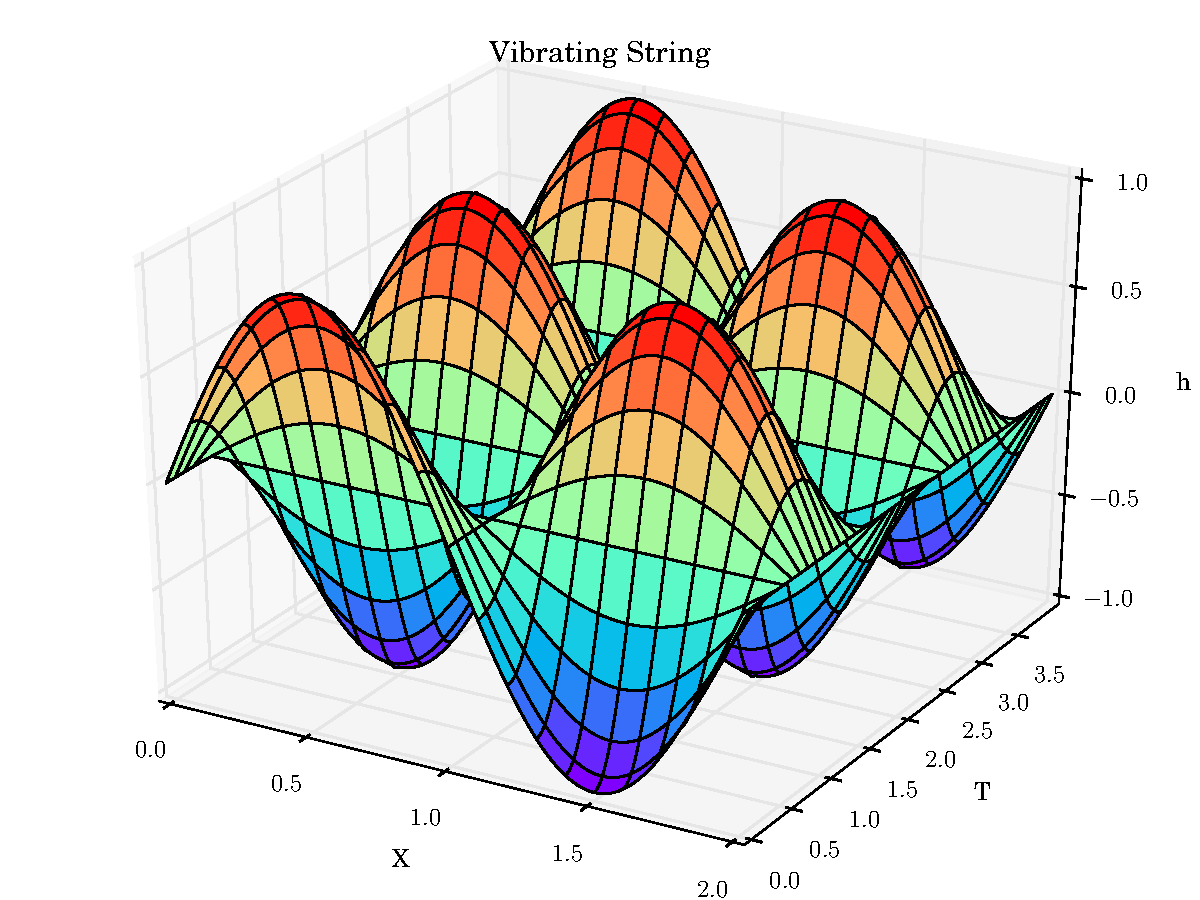
\includegraphics[width=10cm]{3D.pdf}       
\caption{3D graph of the simulation}
\end{figure}

Plot the shape of the string when $t=\{0, 0.5, 1, 1.5, 2\}$:
\begin{python}
	for i in range(5):
	plt.scatter(x,h[i*50,],label="t="+str(i*0.5))
	plt.title(u'Shape of the String',fontsize=14)
	plt.xlabel(u'x',fontsize=14)
	plt.ylabel(u'h',fontsize=14)
	plt.legend(loc='upper left')
	plt.show()
\end{python}

\begin{figure}[htb]
	\centering
	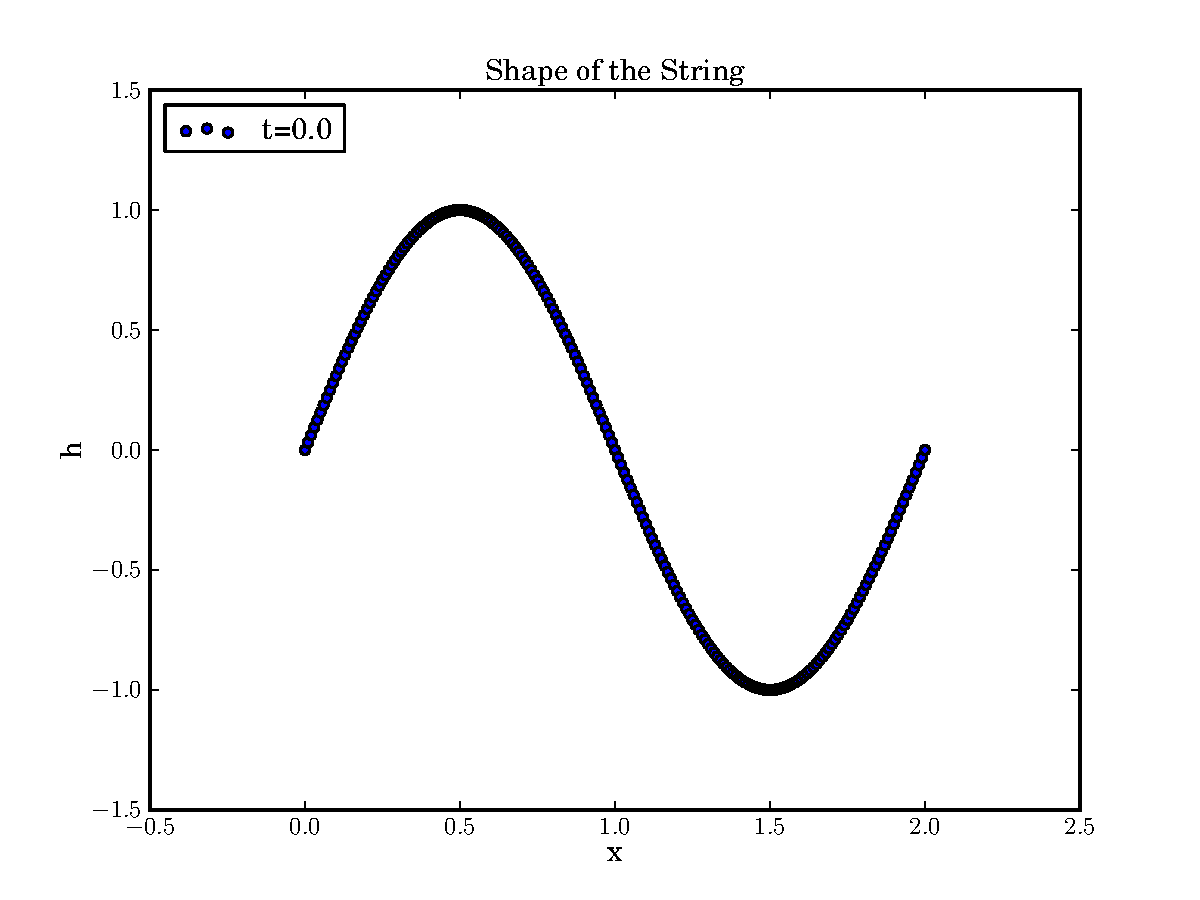
\includegraphics[width=10cm]{t=0.pdf}       
	\caption{Shape of the string when t=0}
\end{figure}

\begin{figure}[htb]
	\centering
	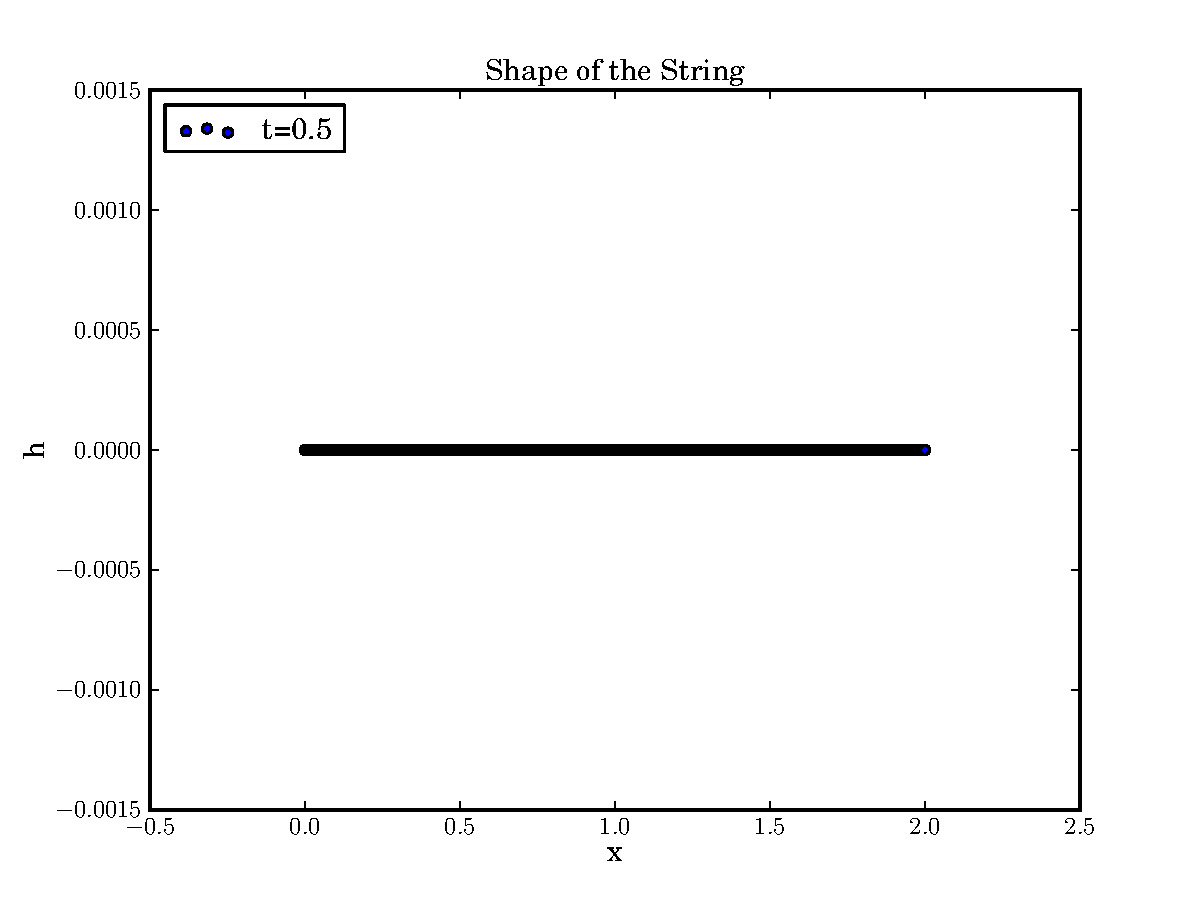
\includegraphics[width=10cm]{t=0_5.pdf}       
	\caption{Shape of the string when t=0.5}
\end{figure}

\begin{figure}[htb]
	\centering
	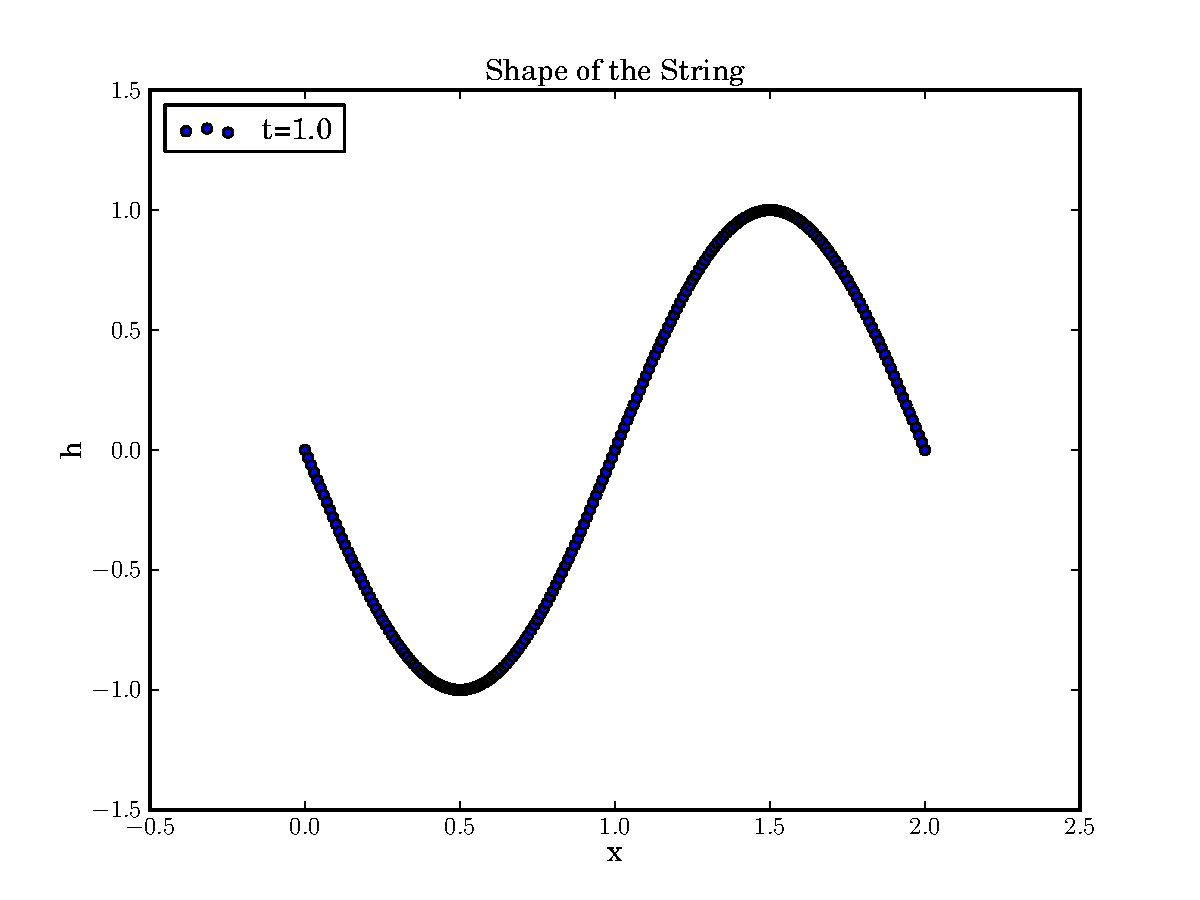
\includegraphics[width=10cm]{t=1.pdf}       
	\caption{Shape of the string when t=1}
\end{figure}

\begin{figure}[htb]
	\centering
	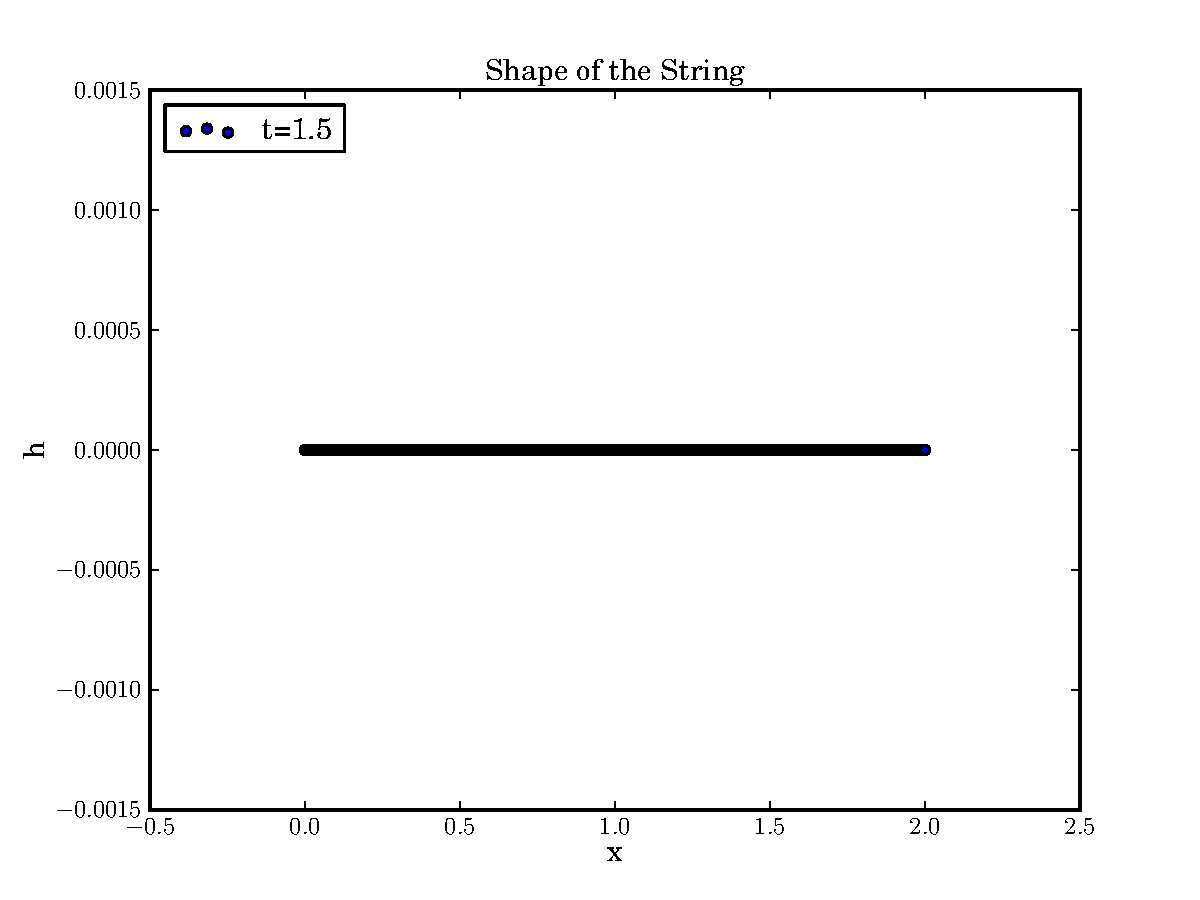
\includegraphics[width=10cm]{t=1_5.pdf}       
	\caption{Shape of the string when t=1.5}
\end{figure}

\begin{figure}[htb]
	\centering
	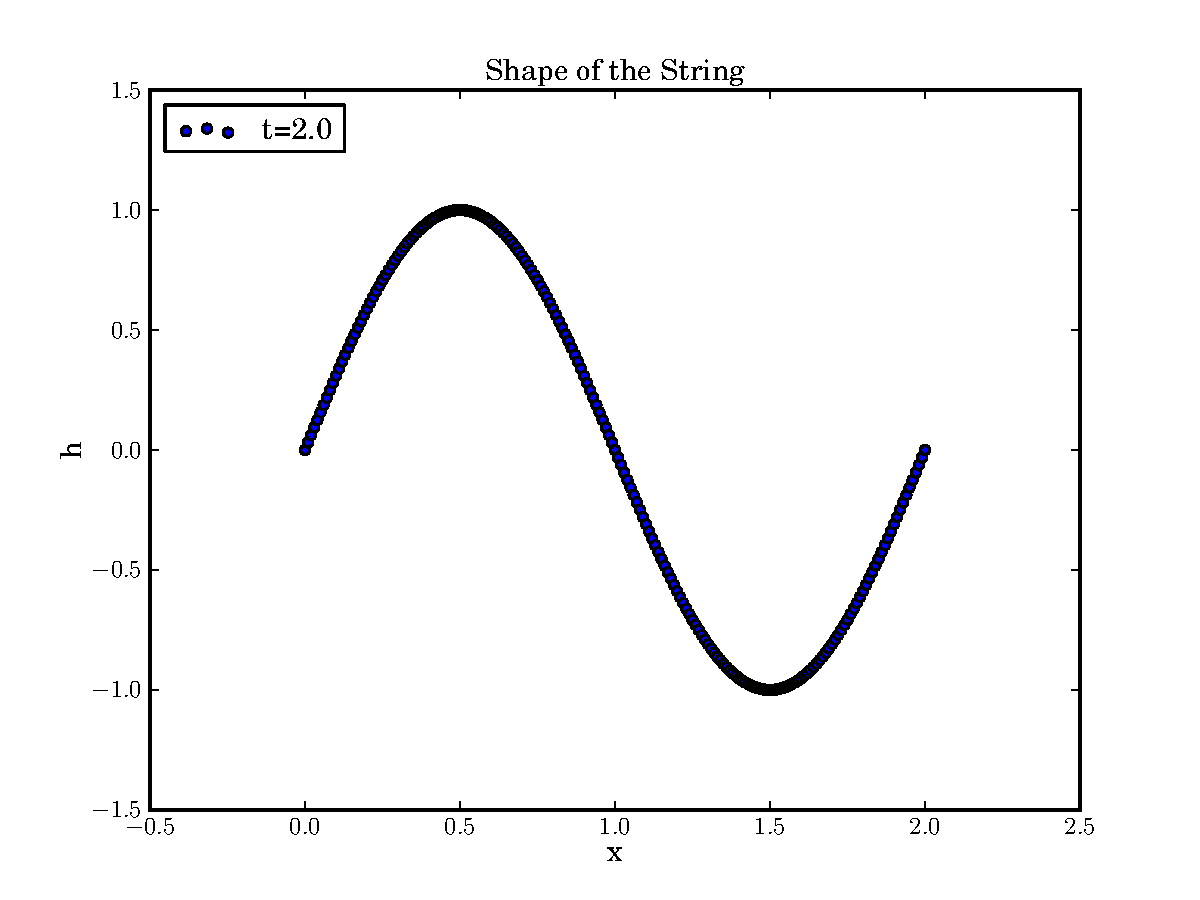
\includegraphics[width=10cm]{t=2.pdf}       
	\caption{Shape of the string when t=2}
\end{figure}
